%iffalse
\let\negmedspace\undefined
\let\negthickspace\undefined
\documentclass[journal,12pt,onecolumn]{IEEEtran}
\usepackage{cite}
\usepackage{amsmath,amssymb,amsfonts,amsthm}
\usepackage{algorithmic}
\usepackage{graphicx}
\usepackage{textcomp}
\usepackage{xcolor}
\usepackage{txfonts}
\usepackage{listings}
\usepackage{enumitem}
\usepackage{mathtools}
\usepackage{gensymb}
\usepackage{comment}
\usepackage[breaklinks=true]{hyperref}
\usepackage{tkz-euclide} 
\usepackage{listings}
\usepackage{gvv}                                        
%\def\inputGnumericTable{}                                 
\usepackage[latin1]{inputenc}     
\usepackage{xparse}
\usepackage{color}                                            
\usepackage{array}                                            
\usepackage{longtable}                                       
\usepackage{calc}                                             
\usepackage{multirow}
\usepackage{multicol}
\usepackage{hhline}                                           
\usepackage{ifthen}                                           
\usepackage{lscape}
\usepackage{tabularx}
\usepackage{array}
\usepackage{float}
\newtheorem{theorem}{Theorem}[section]
\newtheorem{problem}{Problem}
\newtheorem{proposition}{Proposition}[section]
\newtheorem{lemma}{Lemma}[section]
\newtheorem{corollary}[theorem]{Corollary}
\newtheorem{example}{Example}[section]
\newtheorem{definition}[problem]{Definition}
\newcommand{\BEQA}{\begin{eqnarray}}
\newcommand{\EEQA}{\end{eqnarray}}
\usepackage{float}
\usepackage{listings}
\usepackage{xcolor}
%\newcommand{\define}{\stackrel{\triangle}{=}}
\theoremstyle{remark}
\usepackage{ circuitikz }
%\newtheorem{rem}{Remark}
% Marks the beginning of the document
\begin{document}
\title{11.16.3.9}
\author{EE24BTECH11007 - Arnav Makarand Yadnopavit}
\maketitle
\renewcommand{\thefigure}{\theenumi}
\renewcommand{\thetable}{\theenumi}
\parindent 0px Question: If $\frac{1}{12}$ is the probability of an event, what is the probability of the event 'not A'.\\
\solution\\
Let us solve the problem using a Bernouli random variable.

    The Bernoulli R.V is defined as,
\begin{align}
	X_i = \begin{cases}
		0 & \text{not A}\\	
		1 & \text{A}	
	\end{cases}
\end{align}
The PMF of Bernoulli R.V is given by,
\begin{align}
  p_X\brak{x} = \begin{cases}
    1-p & x = 0\\
    p & x = 1
  \end{cases}
\end{align}
\begin{itemize}
    \item The probability of $ A $ occurring is given as $ P(A) = \frac{1}{12} $.  
    Therefore, $ p_X(1) = P(A) = \frac{1}{12} $.

    \item The probability of the complement of $ A $ (denoted as "not $ A $") is $ P(A^\prime) = p_X(0) $. Using the rule of complementary probabilities:
    \[
    P(A^\prime) = 1 - P(A).
    \]

    \item Substitute $ P(A) = \frac{1}{12} $ into the equation:
    \[
    P(A^\prime) = 1 - \frac{1}{12} = \frac{11}{12}.
    \]
\end{itemize}

Thus, the probabilities for the Bernoulli random variable $ X $ are:
The PMF of Bernoulli R.V is given by,
\begin{align}
  p_X\brak{x} = \begin{cases}
    \frac{11}{12} & x = 0\\
    \frac{1}{12} & x = 1
  \end{cases}
\end{align}
Hence probability of the event 'not A' is $\frac{11}{12}$.\\
\textbf{Stem Plot of the PMF}\\
Below is the stem plot for the PMF of the Bernoulli random variable:
\begin{figure}[h]
    \centering
    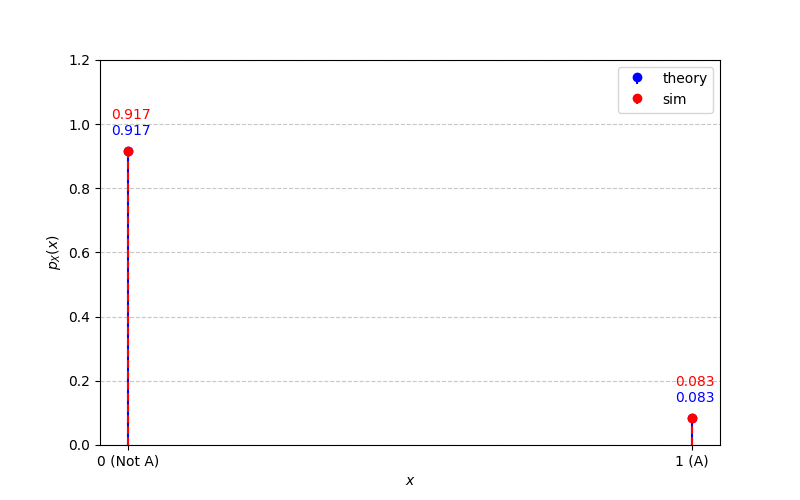
\includegraphics[width=\columnwidth]{figs/fig.png}
 \end{figure}
\end{document}
